\documentclass[11pt]{article}

\usepackage[margin=1in]{geometry}
\usepackage{booktabs}
\usepackage{graphicx}
\usepackage{amsmath}
\usepackage{xeCJK}
\usepackage{hyperref}

\setCJKmainfont{SimSun}
\setmainfont{Times New Roman}

\title{Focus Confidence 与 Glare Risk 诊断分支报告}
\author{SRTP Optical Mechanism Analysis}
\date{2026-06-22}

\begin{document}
\maketitle

\section{Research Question}

前几轮原理分支已经确认，反光微结构的仿真采样方式会影响 glare-risk、焦堆亮度统计和 DFF 深度误差。本轮进一步检查一个更接近论文方法设计的问题：哪些无参考诊断图能够识别 DFF 容易失败的位置？

实验使用一个合成微结构高度图作为 ground truth，并采用 8x super-resolution integrated simulation：先在高分辨率网格上生成微表面、法线、眩光风险和焦堆，再通过 block-average 积分到传感器分辨率。随后使用 Laplacian focus measure 做传统 DFF 深度选择，并将绝对高度误差最高的 10\% 像素定义为 DFF failure top10。

\section{Diagnostics}

本轮比较的诊断分数包括几何 glare risk、焦栈过曝持续性和 focus-response confidence。几何分数包括 \texttt{risk\_mean} 和 \texttt{risk\_max}；饱和相关分数包括 \texttt{sat\_persistence} 和 \texttt{bright\_persistence}；焦向置信度分数包括 \texttt{low\_margin}、\texttt{focus\_entropy} 和 \texttt{low\_peak\_strength}。其中 \texttt{focus\_entropy} 表示 focus response 在多个焦层之间的分散程度，\texttt{low\_margin} 表示第一、第二 focus response 峰值之间的竞争强度。

\section{Results}

\begin{table}[htbp]
\centering
\small
\begin{tabular}{lrrrrr}
\toprule
Score & AUC & Effect & Top10 Err. & Rest Err. & Fail Rate \\
\midrule
\texttt{focus\_entropy} & 0.6111 & 0.3826 & 0.0765 & 0.0626 & 0.1434 \\
\texttt{low\_margin} & 0.5907 & 0.3177 & 0.0665 & 0.0637 & 0.1391 \\
\texttt{hybrid\_risk\_entropy} & 0.5372 & 0.0093 & 0.0646 & 0.0640 & 0.0914 \\
\texttt{sat\_persistence} & 0.5061 & 0.0000 & 0.0648 & 0.0639 & 0.1039 \\
\texttt{low\_peak\_strength} & 0.4920 & 0.0132 & 0.0710 & 0.0632 & 0.1125 \\
\texttt{bright\_persistence} & 0.4629 & -0.2971 & 0.0510 & 0.0655 & 0.0238 \\
\texttt{risk\_max} & 0.4458 & -0.1373 & 0.0662 & 0.0638 & 0.0820 \\
\texttt{risk\_mean} & 0.4443 & -0.1140 & 0.0669 & 0.0637 & 0.0801 \\
\bottomrule
\end{tabular}
\caption{Diagnostic scores for identifying top-10\% DFF failure pixels.}
\end{table}

\begin{figure}[htbp]
\centering
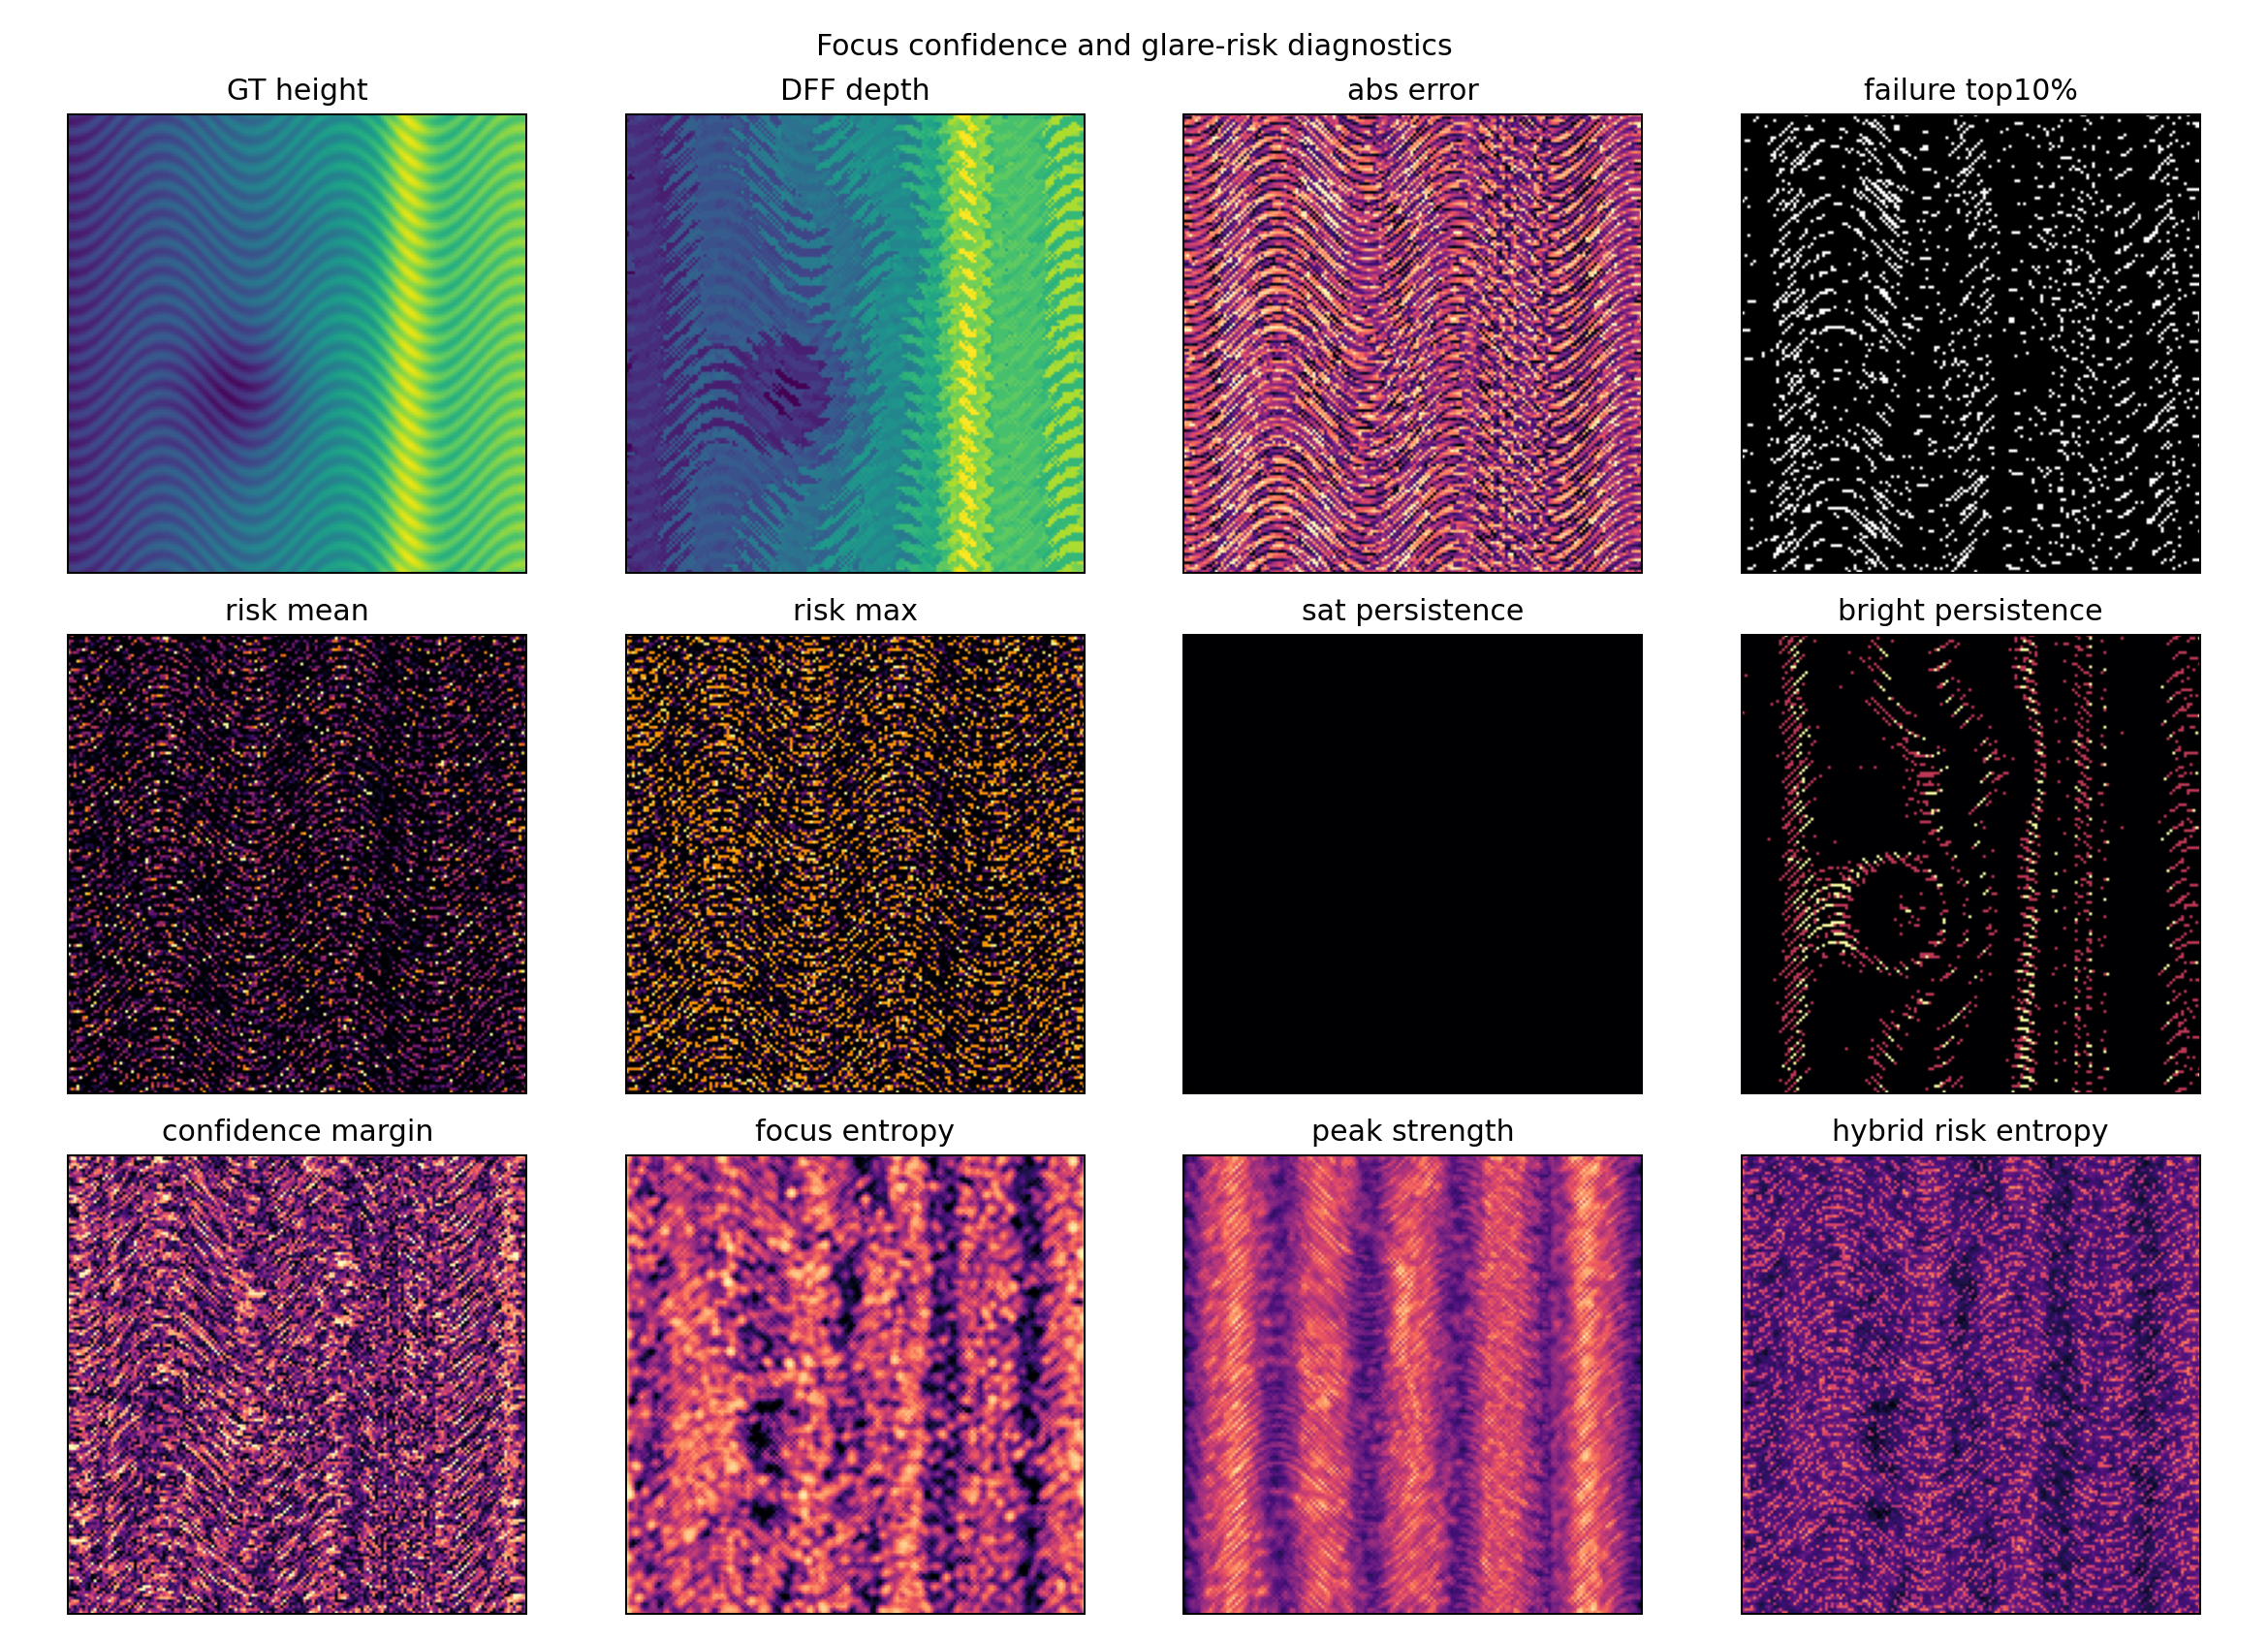
\includegraphics[width=\linewidth]{confidence_risk_branch/confidence_risk_maps.png}
\caption{Focus confidence and glare-risk maps.}
\end{figure}

\begin{figure}[htbp]
\centering
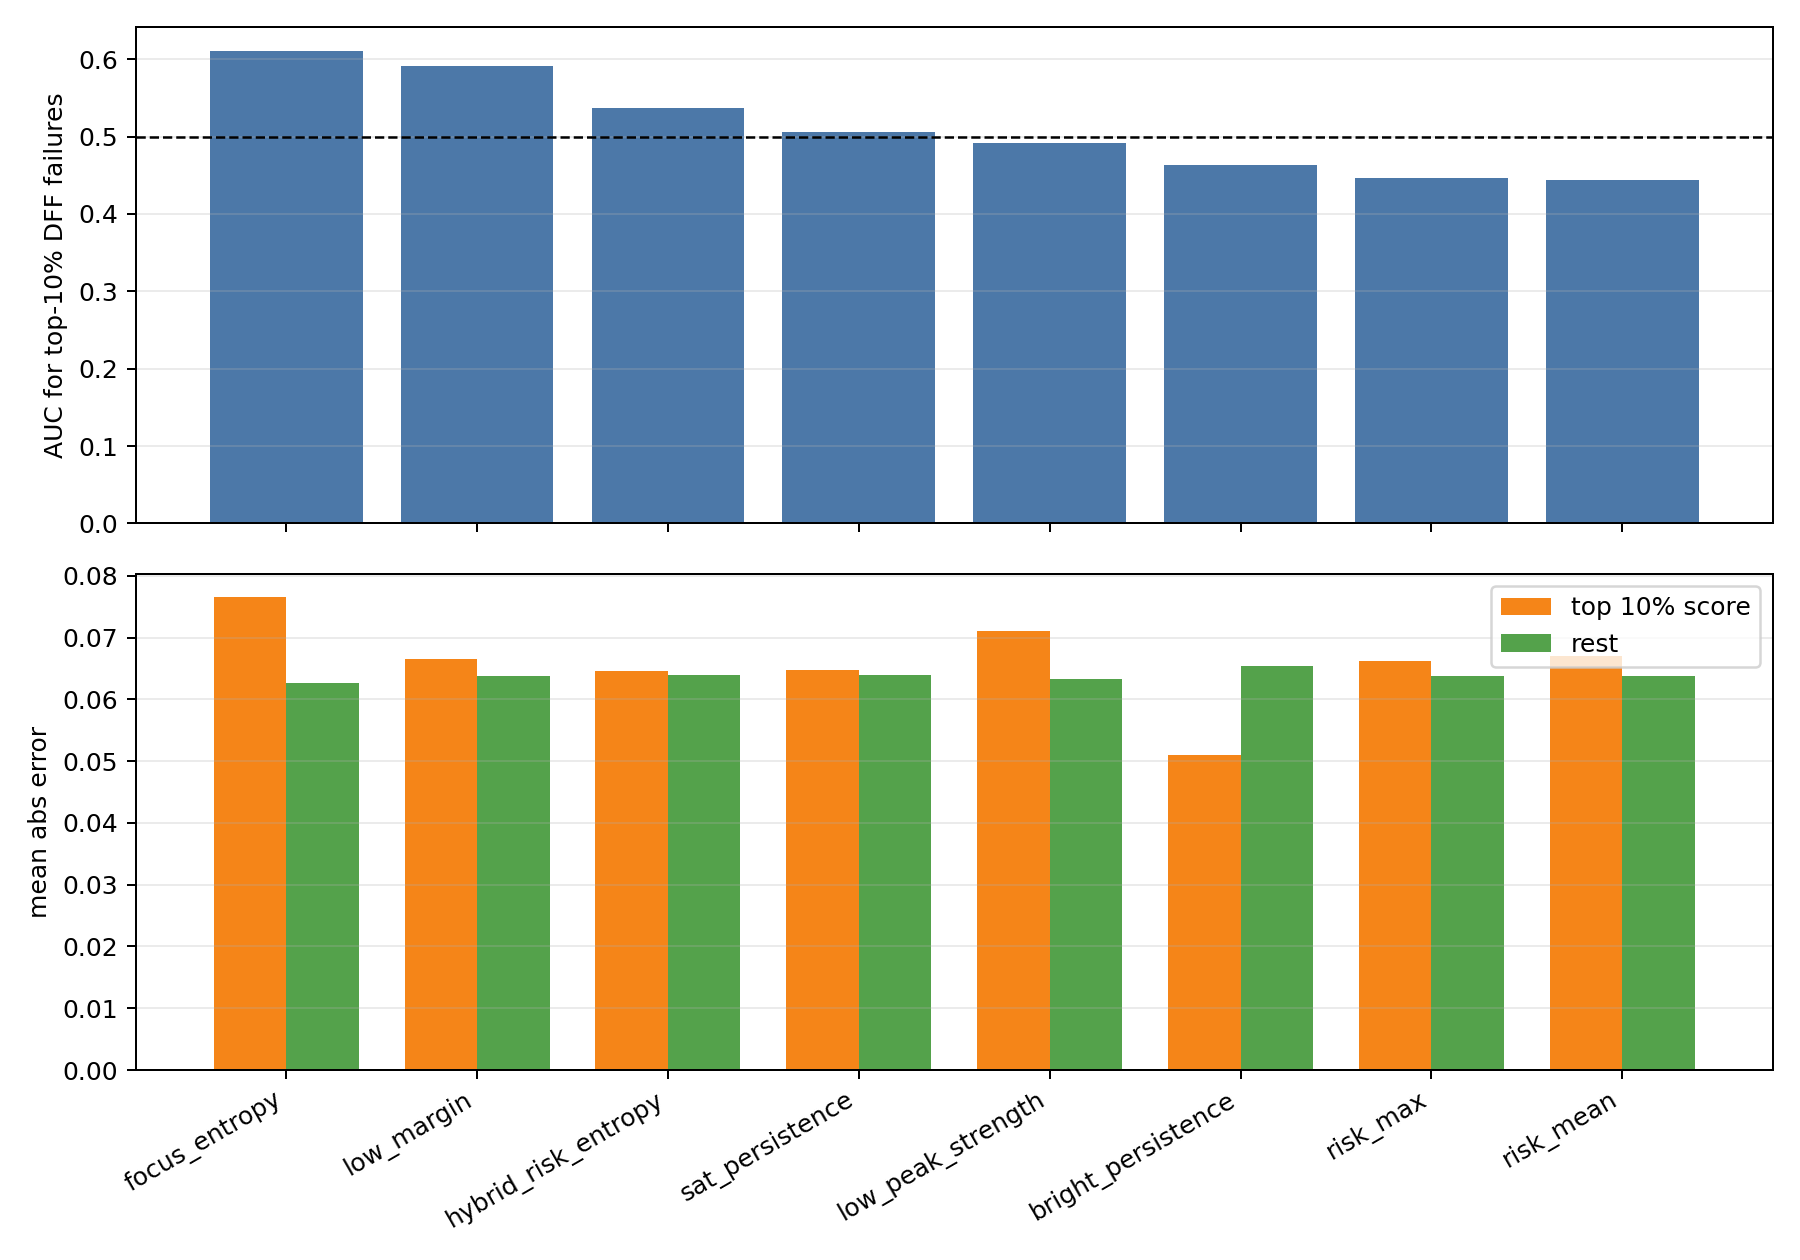
\includegraphics[width=0.86\linewidth]{confidence_risk_branch/confidence_risk_auc_bars.png}
\caption{AUC and error comparison for different diagnostic scores.}
\end{figure}

\section{Key Interpretation}

\texttt{focus\_entropy} is the best single diagnostic in this run, with an AUC of 0.6111 for identifying the top-10\% DFF error pixels. Its top 10\% score region has a mean absolute error of 0.0765, compared with 0.0626 in the remaining region. This result is consistent with the mechanism of DFF: traditional DFF assumes a clear focus-response maximum at each pixel. When reflective artifacts, weak texture, or local saturation create ambiguous or multi-modal focus responses, the argmax depth selection becomes unstable.

\texttt{low\_margin} provides a similar confidence cue, with an AUC of 0.5907 and a failure rate of 13.91\% in its top 10\% score region. It directly measures the competition between the first and second focus-response peaks, making it suitable for confidence masking or loss weighting.

In contrast, \texttt{risk\_mean} and \texttt{risk\_max} perform below random ranking in this synthetic setting. This does not invalidate glare-risk modeling. Instead, it shows that geometric glare risk should not be treated as a direct failure mask. Glare risk describes where reflective artifacts may be generated, while DFF failure also depends on focus ambiguity, texture strength, saturation persistence, local morphology, and sampling.

\section{Method Implication}

The current evidence supports upgrading a single glare-risk prior into a quality-aware prior:

\begin{equation}
Q_{\mathrm{fail}}(x) =
\alpha H_{\mathrm{focus}}(x)
+ \beta (1 - M_{\mathrm{focus}}(x))
+ \gamma P_{\mathrm{sat}}(x)
+ \delta R_{\mathrm{glare}}(x),
\end{equation}

where $H_{\mathrm{focus}}$ denotes focus entropy, $M_{\mathrm{focus}}$ denotes focus margin, $P_{\mathrm{sat}}$ denotes saturation persistence, and $R_{\mathrm{glare}}$ denotes geometric glare risk. The weights should be calibrated on synthetic validation data or a small set of manually inspected ROIs.

The quality map can be used for weighted supervision:

\begin{equation}
\mathcal{L} =
\mathrm{mean}\left((1 + \lambda Q_{\mathrm{fail}}) \cdot
\left|H_{\mathrm{pred}} - H_{\mathrm{gt}}\right|\right).
\end{equation}

This training strategy encourages the model to focus on reflective pseudo-edges, focus ambiguity, and locally saturated regions rather than only minimizing average reconstruction error.

\section{Paper-Ready Statement}

To avoid treating geometric glare risk as a direct error mask, we further analyze the reliability of the focus response itself. For each pixel, we compute focus-response entropy, top-2 focus margin, and saturation persistence, and evaluate their ability to identify the top 10\% DFF error pixels. In the synthetic super-resolution-integrated stack, focus entropy provides the strongest single diagnostic, with an AUC of 0.6111. Pixels in the top 10\% entropy region exhibit a mean absolute error of 0.0765, compared with 0.0626 in the remaining region. This result suggests that DFF failures are not determined by glare-prone geometry alone; they are more directly associated with ambiguous or multi-modal focus responses. We therefore combine flare-risk priors with focus-confidence priors for loss weighting, failure-region diagnosis, and no-reference quality assessment on real focus stacks.

\section{Next Steps}

The current result should be repeated across multiple random microstructures, roughness levels, exposure settings, and reflection strengths. The same diagnostics should also be computed on real focus-stack ROIs to check whether focus entropy and low margin align with visible pseudo-edges, saturated rims, and DFF spikes. Finally, the proposed quality map should be connected to training or post-processing to verify whether it reduces high-risk MAE, P90 error, and spike count.

\end{document}
